\documentclass{beamer}

\usepackage[utf8]{inputenc}
\usepackage{amssymb}
\usepackage{graphicx}
\usepackage{amsmath}

%% Title page formatting
\title{Tree cover variability increases from 2005 to 2100\\ in Sub-Saharan Africa}
\author{Eric Kalosa-Kenyon, Cody Carroll, Amy Kim}
\institute{University of California, Davis}
\date{}

\begin{document}

\frame{\titlepage}

\begin{frame}
    \frametitle{Introduction: climate system}
    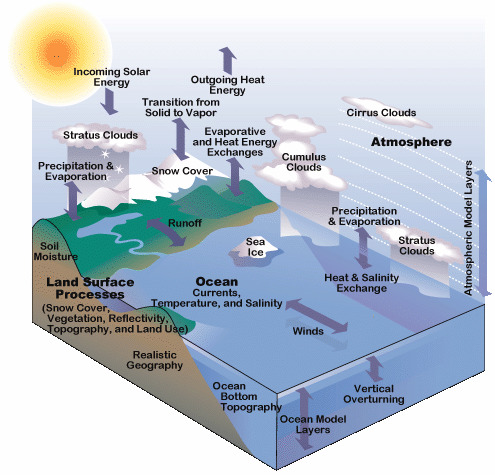
\includegraphics[height=3in]{../img/ccsm_diagram_picture.jpeg}

    https://www.ucar.edu/communications/CCSM/overview.html
\end{frame}

\begin{frame}
    \frametitle{Introduction: climate system modeling}
    \begin{itemize}
        \item Climate change is driven by anthropogenic carbon forcing
        \item IPCC has developed representative carbon forcing trajectories
        \item Computer simulations are run predicated on particular forcing
            pathways
        \item These simulations are realizations of gridded meteorological PDEs
    \end{itemize}
    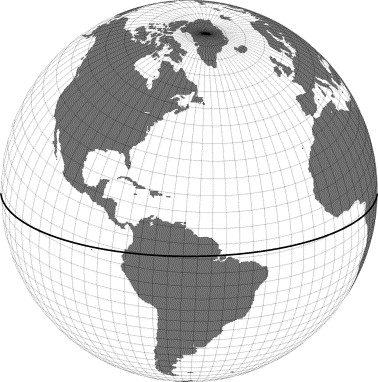
\includegraphics[width=\textwidth/2]{../img/greenland_pole_grid.jpg}
\end{frame}

\begin{frame}
    \frametitle{Introduction: climate system modeling}
    \begin{itemize}
        \item The Community Climate Model System has 5 components and a coupler:
            atmosphere, sea, land, sea ice, and land ice.
        \item We focus on the land system output from a single ensemble under
            the RCP4.5 experiment.

        \item $\theta\in\Theta, \{X_t|t\in\mathbb{Z}\} \textrm{ where }
            X_t\sim \textrm{ARMA}_\theta$
    \end{itemize}
\end{frame}

\begin{frame}
    \frametitle{Introduction: leaf area index (LAI)}
    \begin{columns}

        \column{2in}
            \begin{itemize}
                \item LAI is unitless quantity (leaf area ($m^2$))/(ground area ($m^2$))
                \item "Comparative Physiological Studies on the Growth of Field Crops" Watson 1947 Annals of Botany
                \item Bounded below by 0, above by physiological limits
                \item We interrogate a location in a tropical rainforest
            \end{itemize}

        \column{3in}
            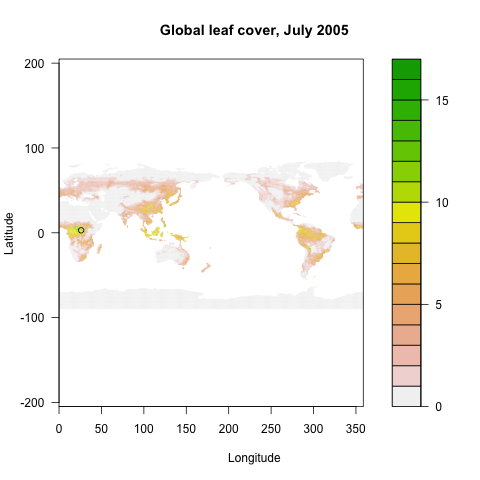
\includegraphics[height=3in]{../img/LAI_global_t0.png}

    \end{columns}
\end{frame}


\begin{frame}
    \frametitle{Raw data}
    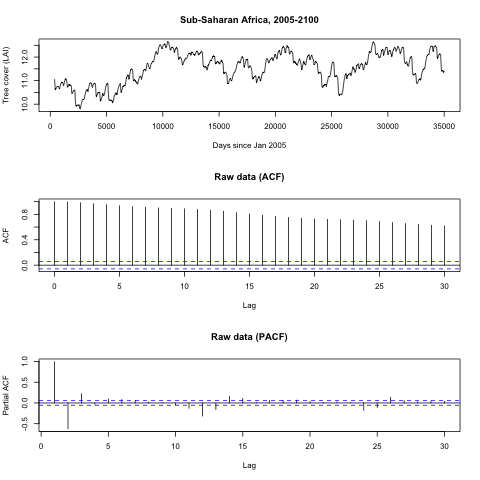
\includegraphics[height=3in]{../img/pacf_acf_raw.png}
\end{frame}

\begin{frame}
    \frametitle{Detrended data}
    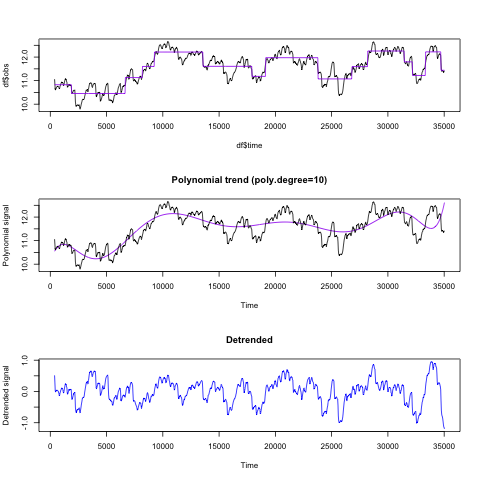
\includegraphics[height=3in]{../img/detrended_acf_pacf.png}
\end{frame}

\begin{frame}
    \frametitle{Standardize variance}
    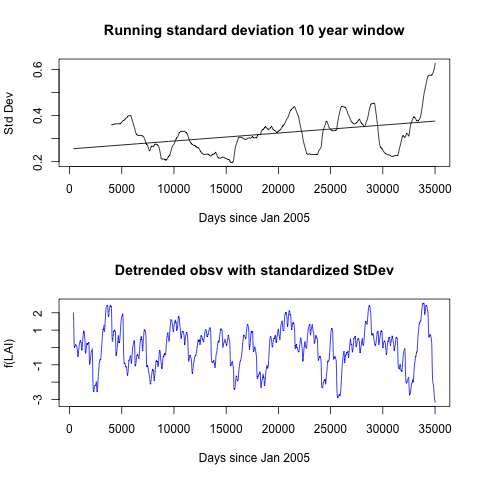
\includegraphics[height=3in]{../img/standatdized_var_LAI.png}
\end{frame}

\begin{frame}
    \frametitle{Standardized variance}
    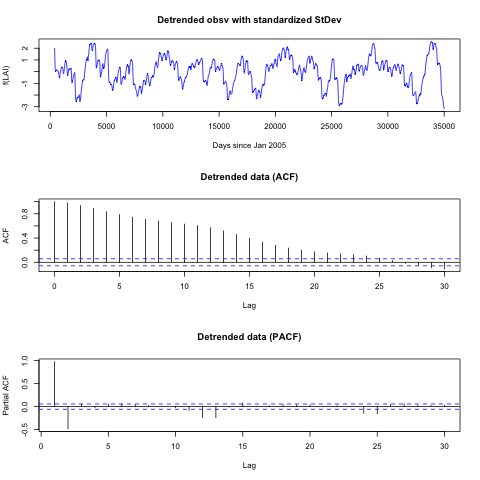
\includegraphics[height=3in]{../img/detrended_stdzd_acf_pacf.png}
\end{frame}

\begin{frame}
    \frametitle{Differenced data}
    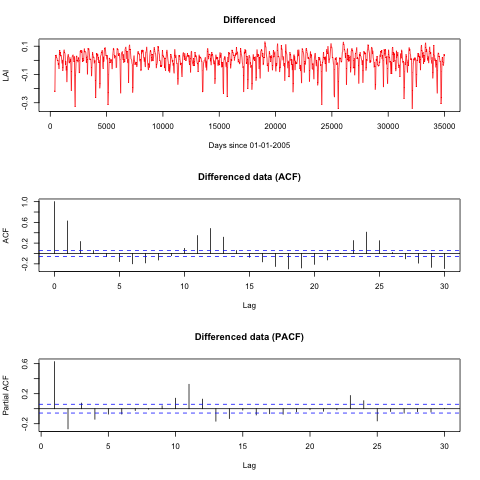
\includegraphics[height=3in]{../img/differenced_acf_pacf.png}
    Perhaps we need to deseason the data before differencing to find
    stationarity.
\end{frame}

\begin{frame}
    \frametitle{Deseasonized data}
    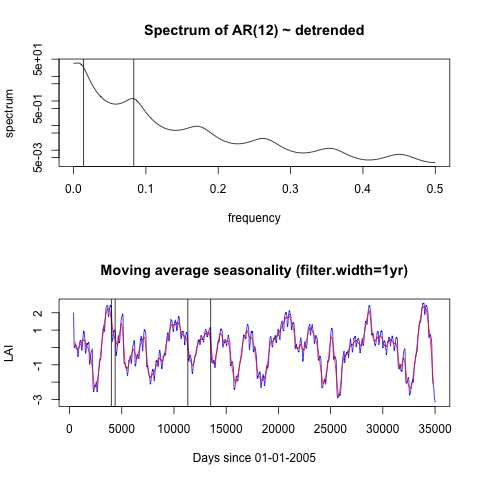
\includegraphics[height=3in]{../img/deseasonalization_spectrum.png}
\end{frame}

\begin{frame}
    \frametitle{Deseasonized data}
    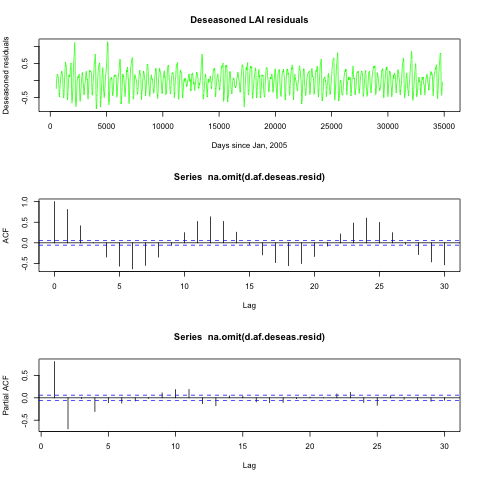
\includegraphics[height=3in]{../img/deseasonalization_resid.png}
\end{frame}

\begin{frame}
    \frametitle{Deseasonized data}
    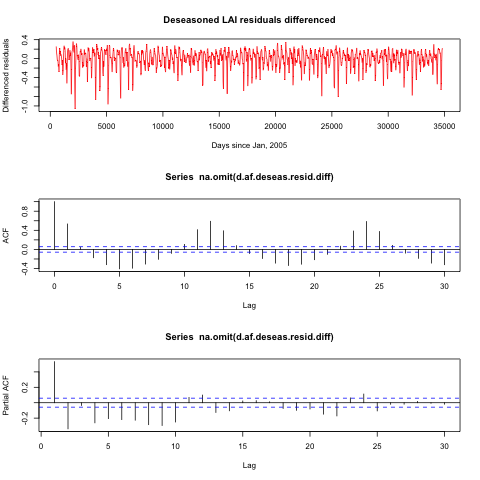
\includegraphics[height=3in]{../img/deseasonalization_resid_difference.png}
\end{frame}

\begin{frame}
    \frametitle{Deseasonized data}
    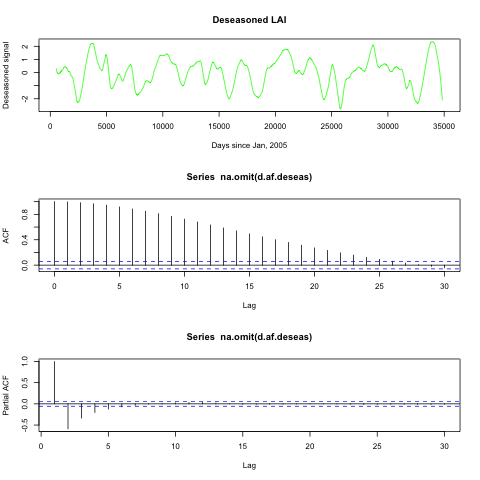
\includegraphics[height=3in]{../img/deseasonalization.png}
\end{frame}

\begin{frame}
    \frametitle{AR(4)}
    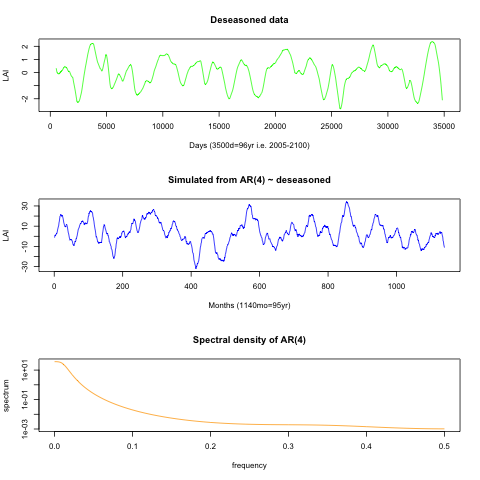
\includegraphics[height=3in]{../img/ar_sim.png}
\end{frame}

\begin{frame}
\frametitle{Principal Component Analysis}
\begin{itemize}
	\item 12818 locations, 1140 time points
	\item $\mathbf{Z}(s,t) = \mathbf{U}\mathbf{\Lambda}\mathbf{V}^T$  
	\item $\mathbf{Z}(s,t)  = \begin{pmatrix}
	z(s_1, t_1) & z(s_2, t_1) & z(s_3, t_1) & \dots & z(s_{12818}, t_1) \\
	z(s_1, t_2) & z(s_2, t_2) & z(s_3, t_2) & \dots & z(s_{12818}, t_2) \\
	\vdots & \vdots & \vdots & \ddots & \vdots\\
	z(s_1, t_{1140}) & z(s_2, t_{1140}) & z(s_3, t_{1140}) & \dots & z(s_{12818}, t_{1140})\\ 
	\end{pmatrix}$
\end{itemize}
\end{frame}


\begin{frame}
\frametitle{Principal Component Analysis}
\begin{columns}
	\column{2in}
	\begin{table}[ht]
		\begin{figure}
			\centering
			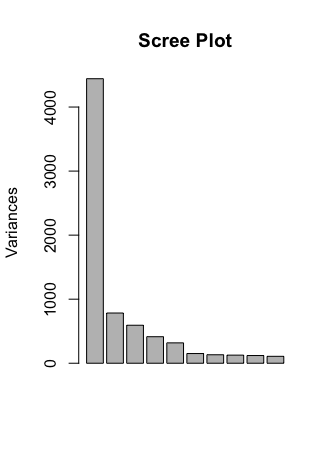
\includegraphics[height=0.7\textheight]{../img/Scree_plot1}
			\caption{Raw Data}
			\label{fig:screeplot1}
		\end{figure}
	\end{table}
	\column{2in}
	\begin{table}[ht]
	\begin{figure}
		\centering
		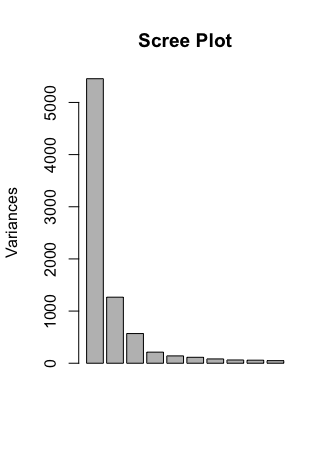
\includegraphics[height=0.7\textheight]{../img/Scree_plot2}
		\caption{Detrend Data}
		\label{fig:screeplot2}
	\end{figure}
\end{table}
		
\end{columns}
\end{frame}

\begin{frame}
\frametitle{Principal Component Analysis}
\begin{table}[ht]
	\centering
	\begin{tabular}{rrrrrrr}
		\hline
		& PC1 & PC2 & PC3 & PC4 & PC5 & PC6 \\ 
		\hline
		SD & 66.650 & 28.003 & 24.356 & 20.348 & 17.832 & 12.301 \\ 
		Prop. of Var. & 0.347 & 0.061 & 0.046 & 0.032 & 0.025 & 0.012 \\ 
		Cum. Prop.& 0.347 & 0.408 & 0.454 & 0.486 & 0.511 & 0.523 \\ 
		\hline
	\end{tabular}
\end{table}
\begin{table}[ht]
	\centering
	\begin{tabular}{rrrrrrr}
		\hline
		& PC1 & PC2 & PC3 & PC4 & PC5 & PC6 \\ 
		\hline
		SD & 73.857 & 35.586 & 23.852 & 14.581 & 11.859 & 10.669 \\ 
		Prop. of Var. & 0.426 & 0.099 & 0.044 & 0.017 & 0.011 & 0.009 \\ 
		Cum. Prop. & 0.426 & 0.524 & 0.569 & 0.585 & 0.596 & 0.605 \\ 
		\hline
	\end{tabular}
\end{table}
\end{frame}

\begin{frame}
\frametitle{Principal Component Analysis}
\begin{figure}
	\centering
	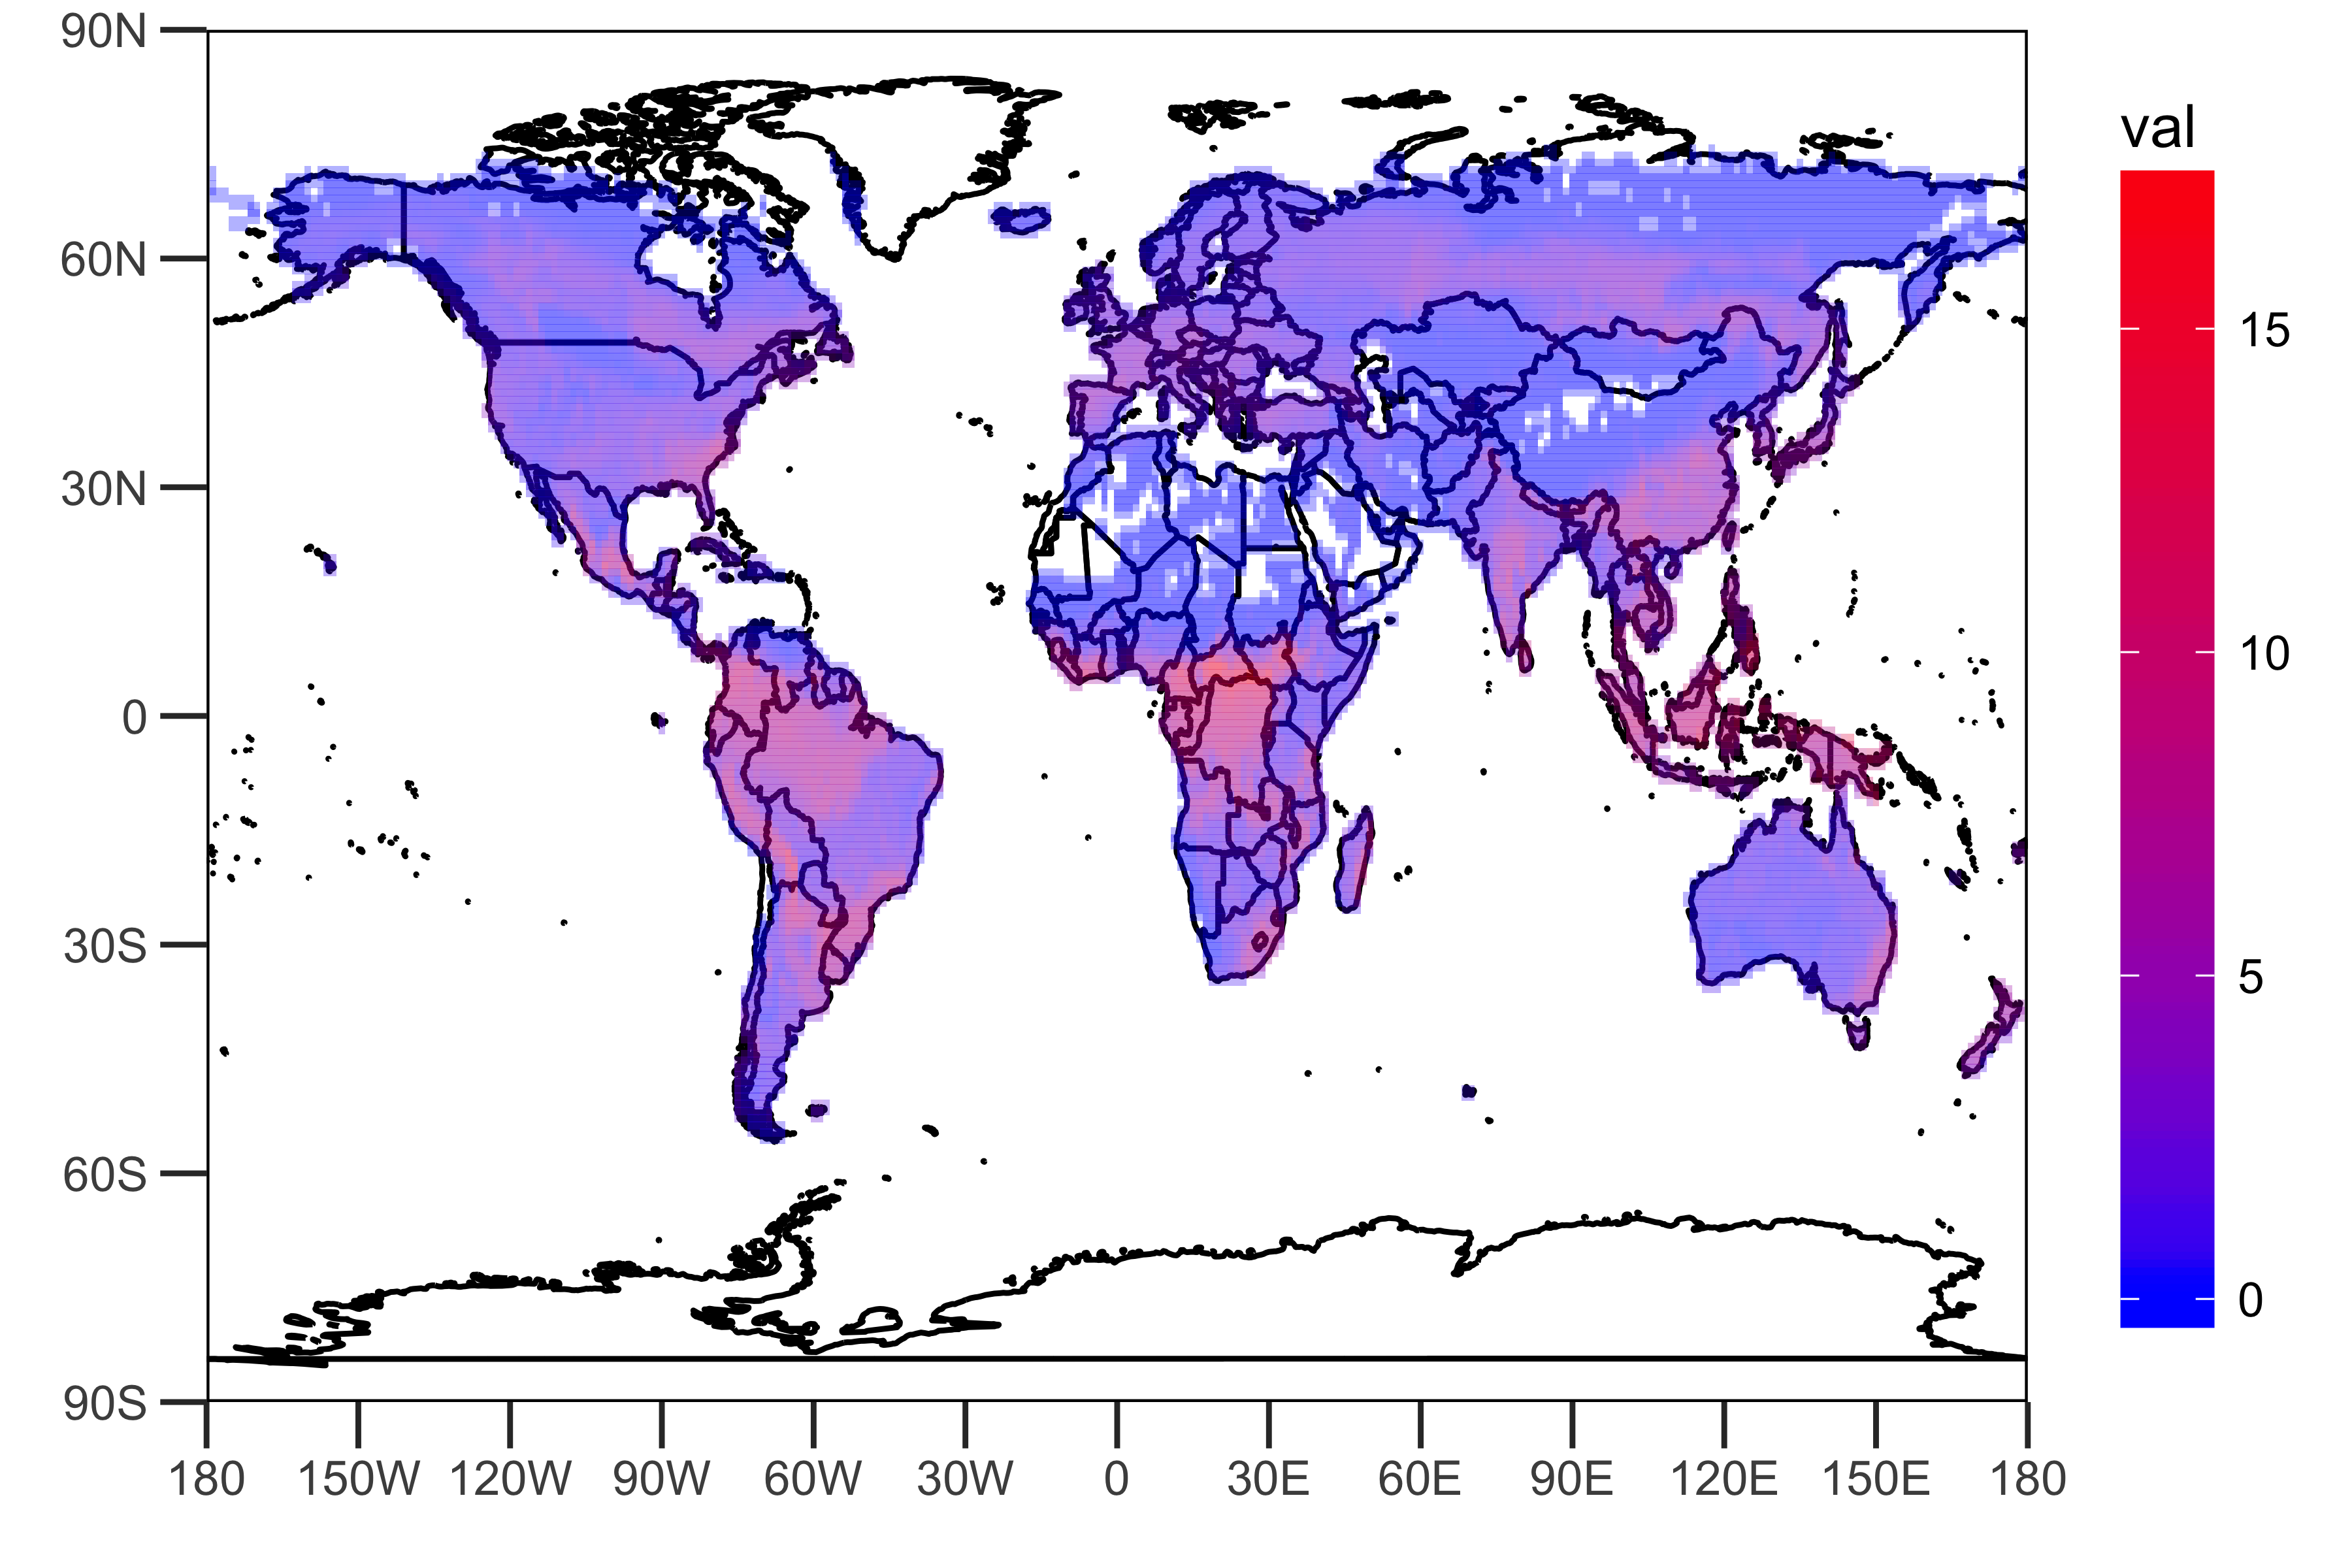
\includegraphics[width=0.9\linewidth]{../img/sample_plot}
	\caption{Global Leaf Index at Time 1}
	\label{fig:sampleplot}
\end{figure}

\end{frame}


\begin{frame}
\frametitle{Principal Component Analysis}
\begin{figure}
	\centering
	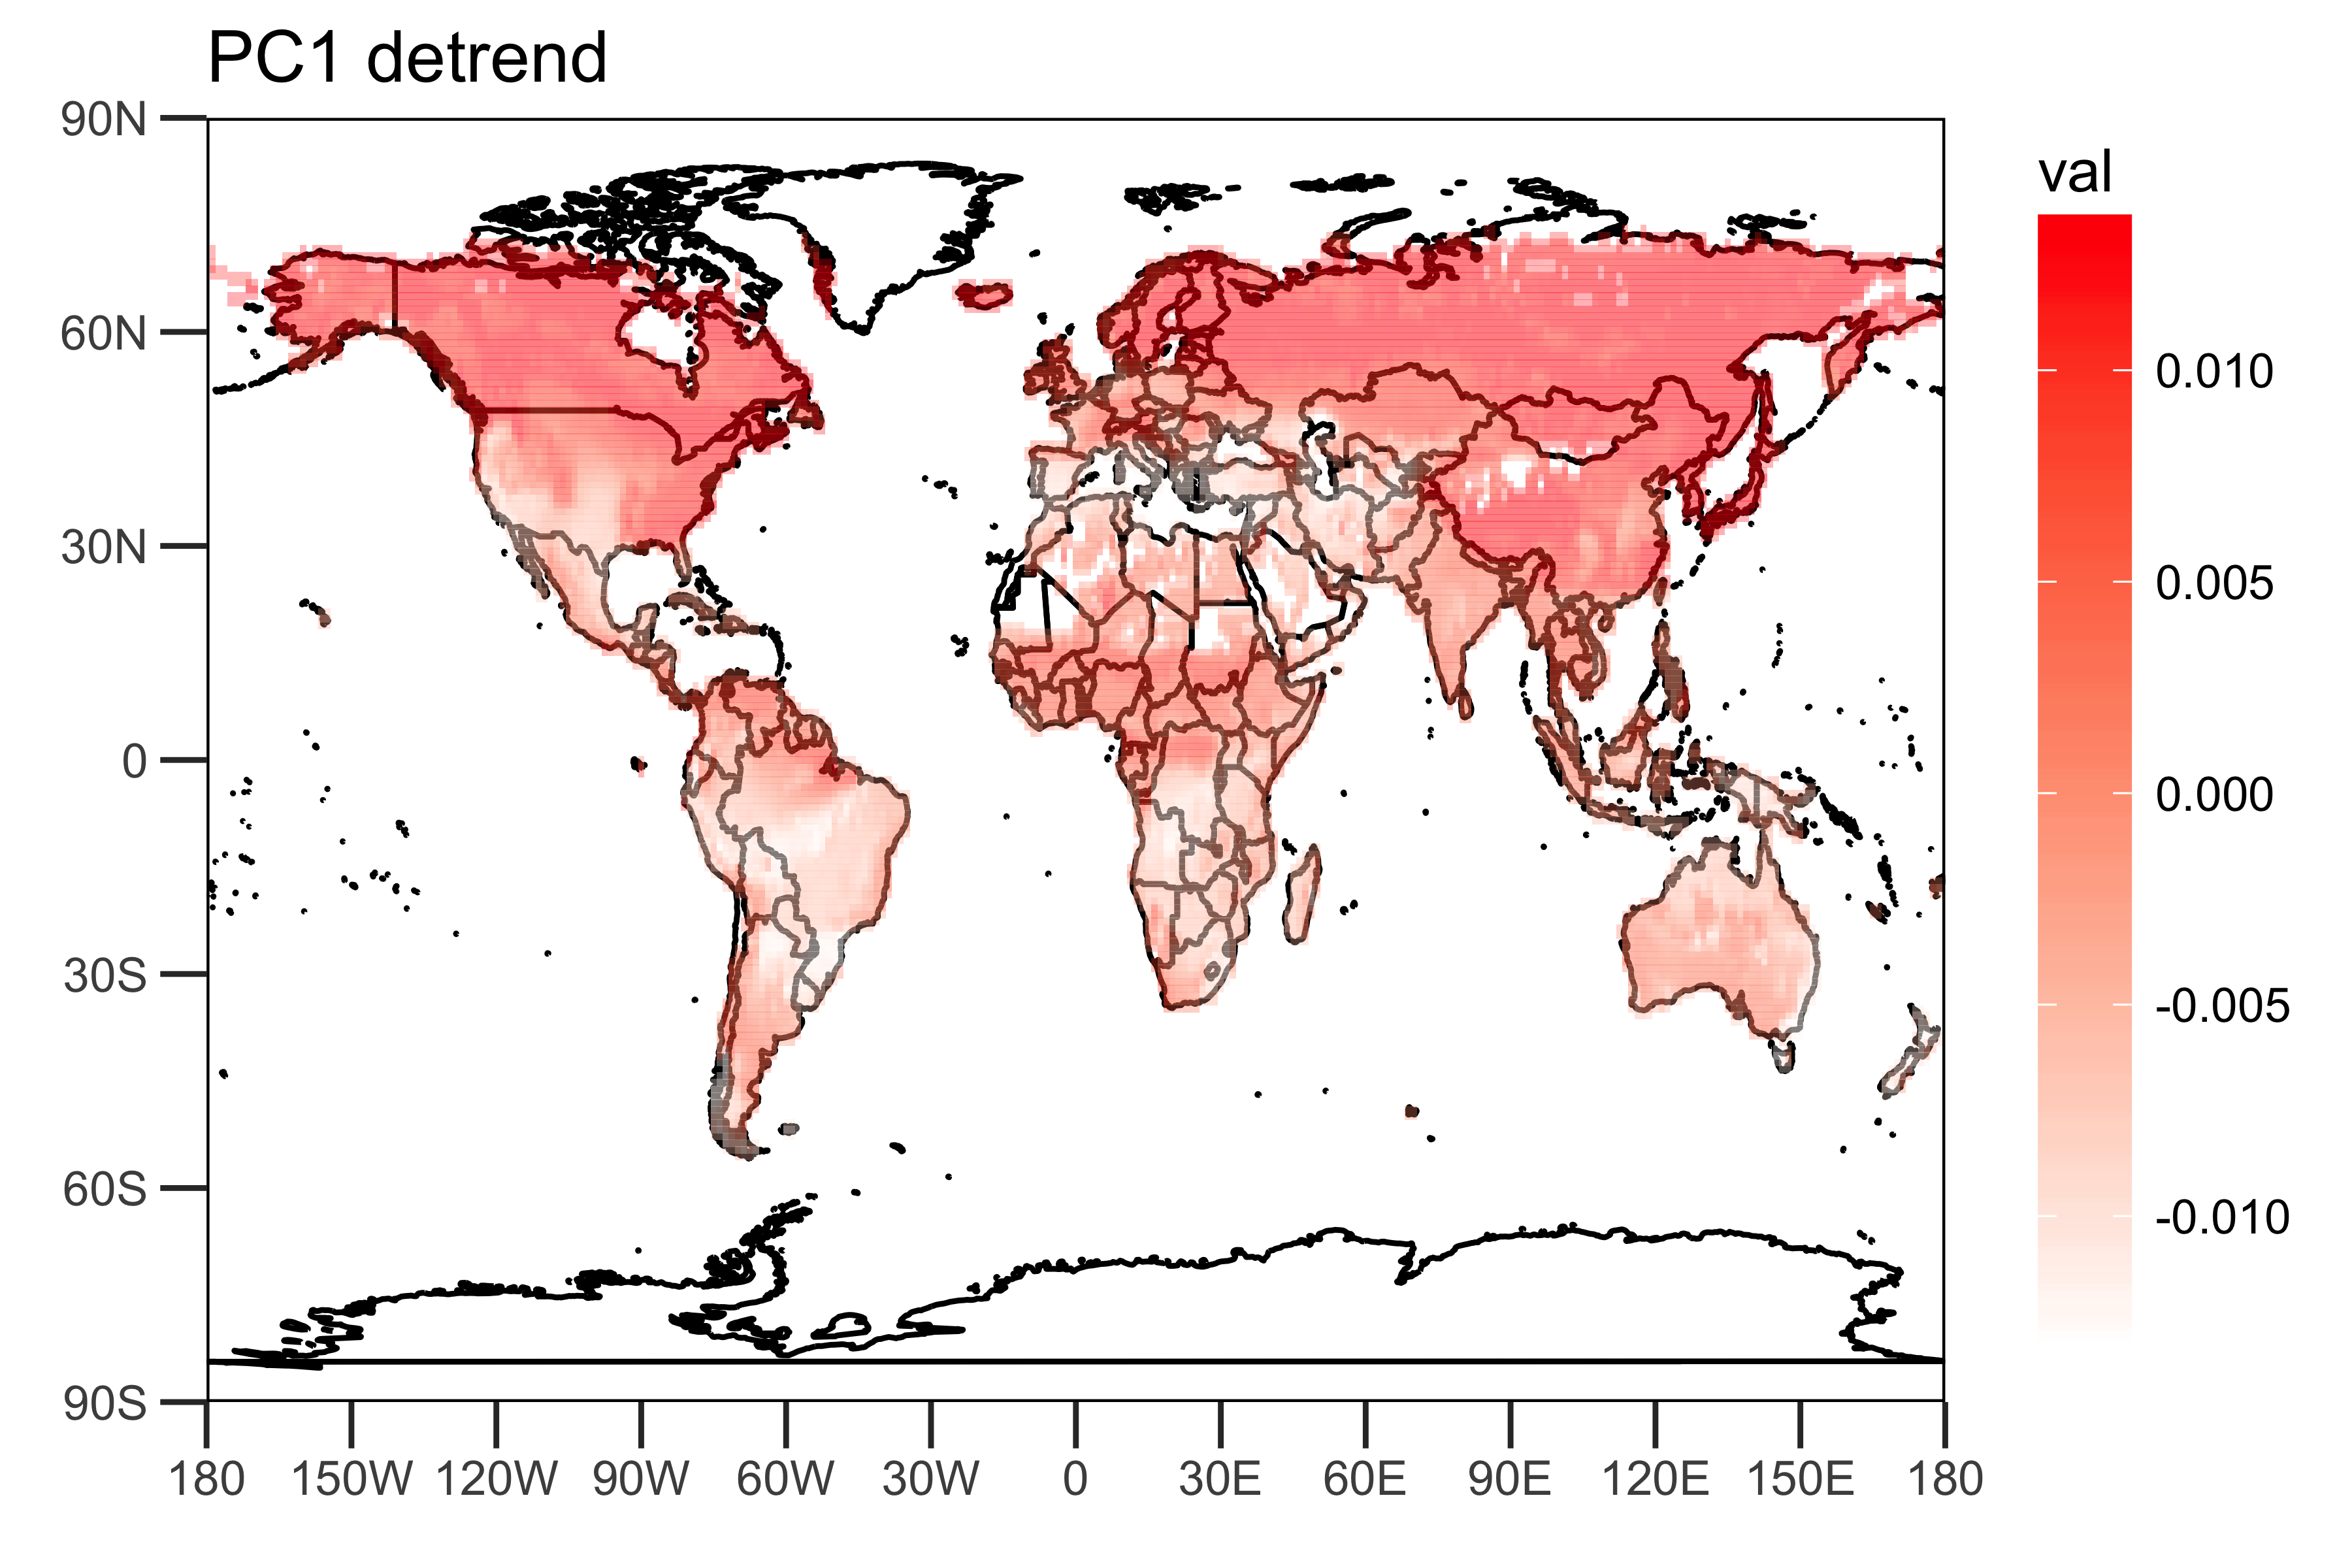
\includegraphics[width=0.9\linewidth]{../img/loading_PC1_de}
	\caption{Loadings of Principal Component 1}
	\label{fig:loadingpc1}
\end{figure}
\end{frame}

\begin{frame}
\frametitle{Principal Component Analysis}
\begin{figure}
	\centering
	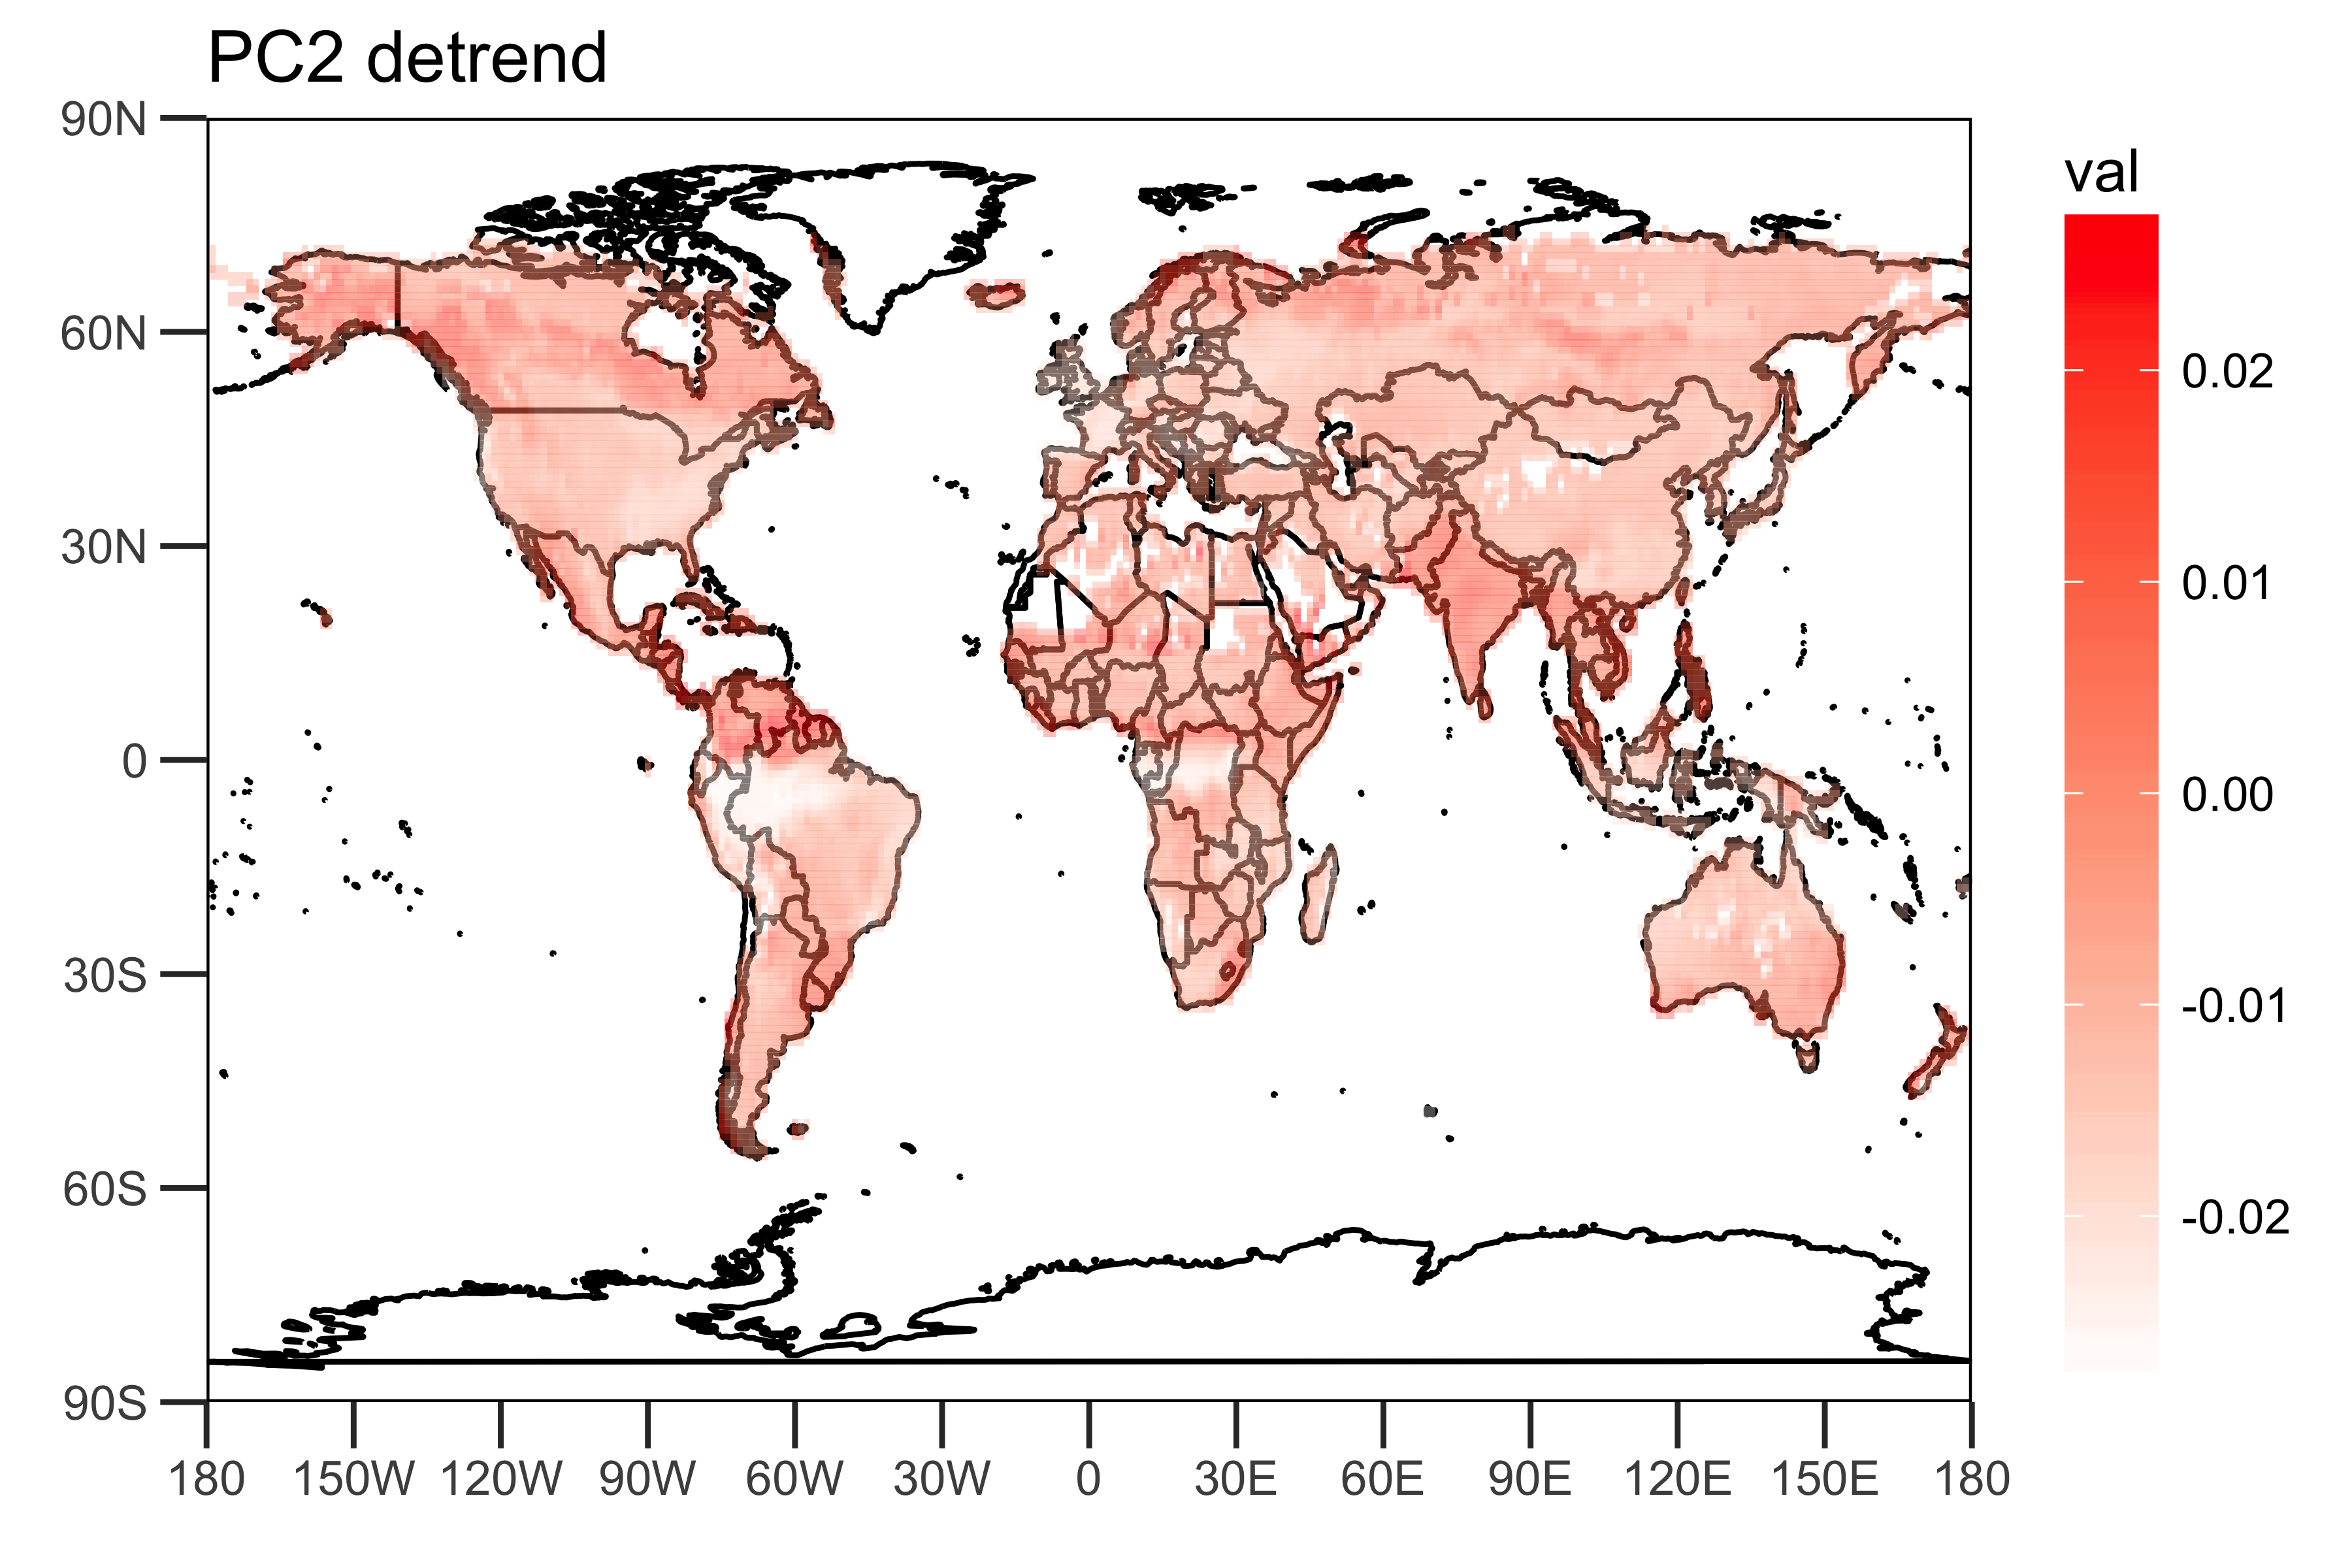
\includegraphics[width=0.9\linewidth]{../img/loading_PC2_de}
	\caption{Loadings of Principal Component 2}
	\label{fig:loadingpc2}
\end{figure}
\end{frame}

\begin{frame}
\frametitle{Principal Component Analysis}
\begin{figure}
	\centering
	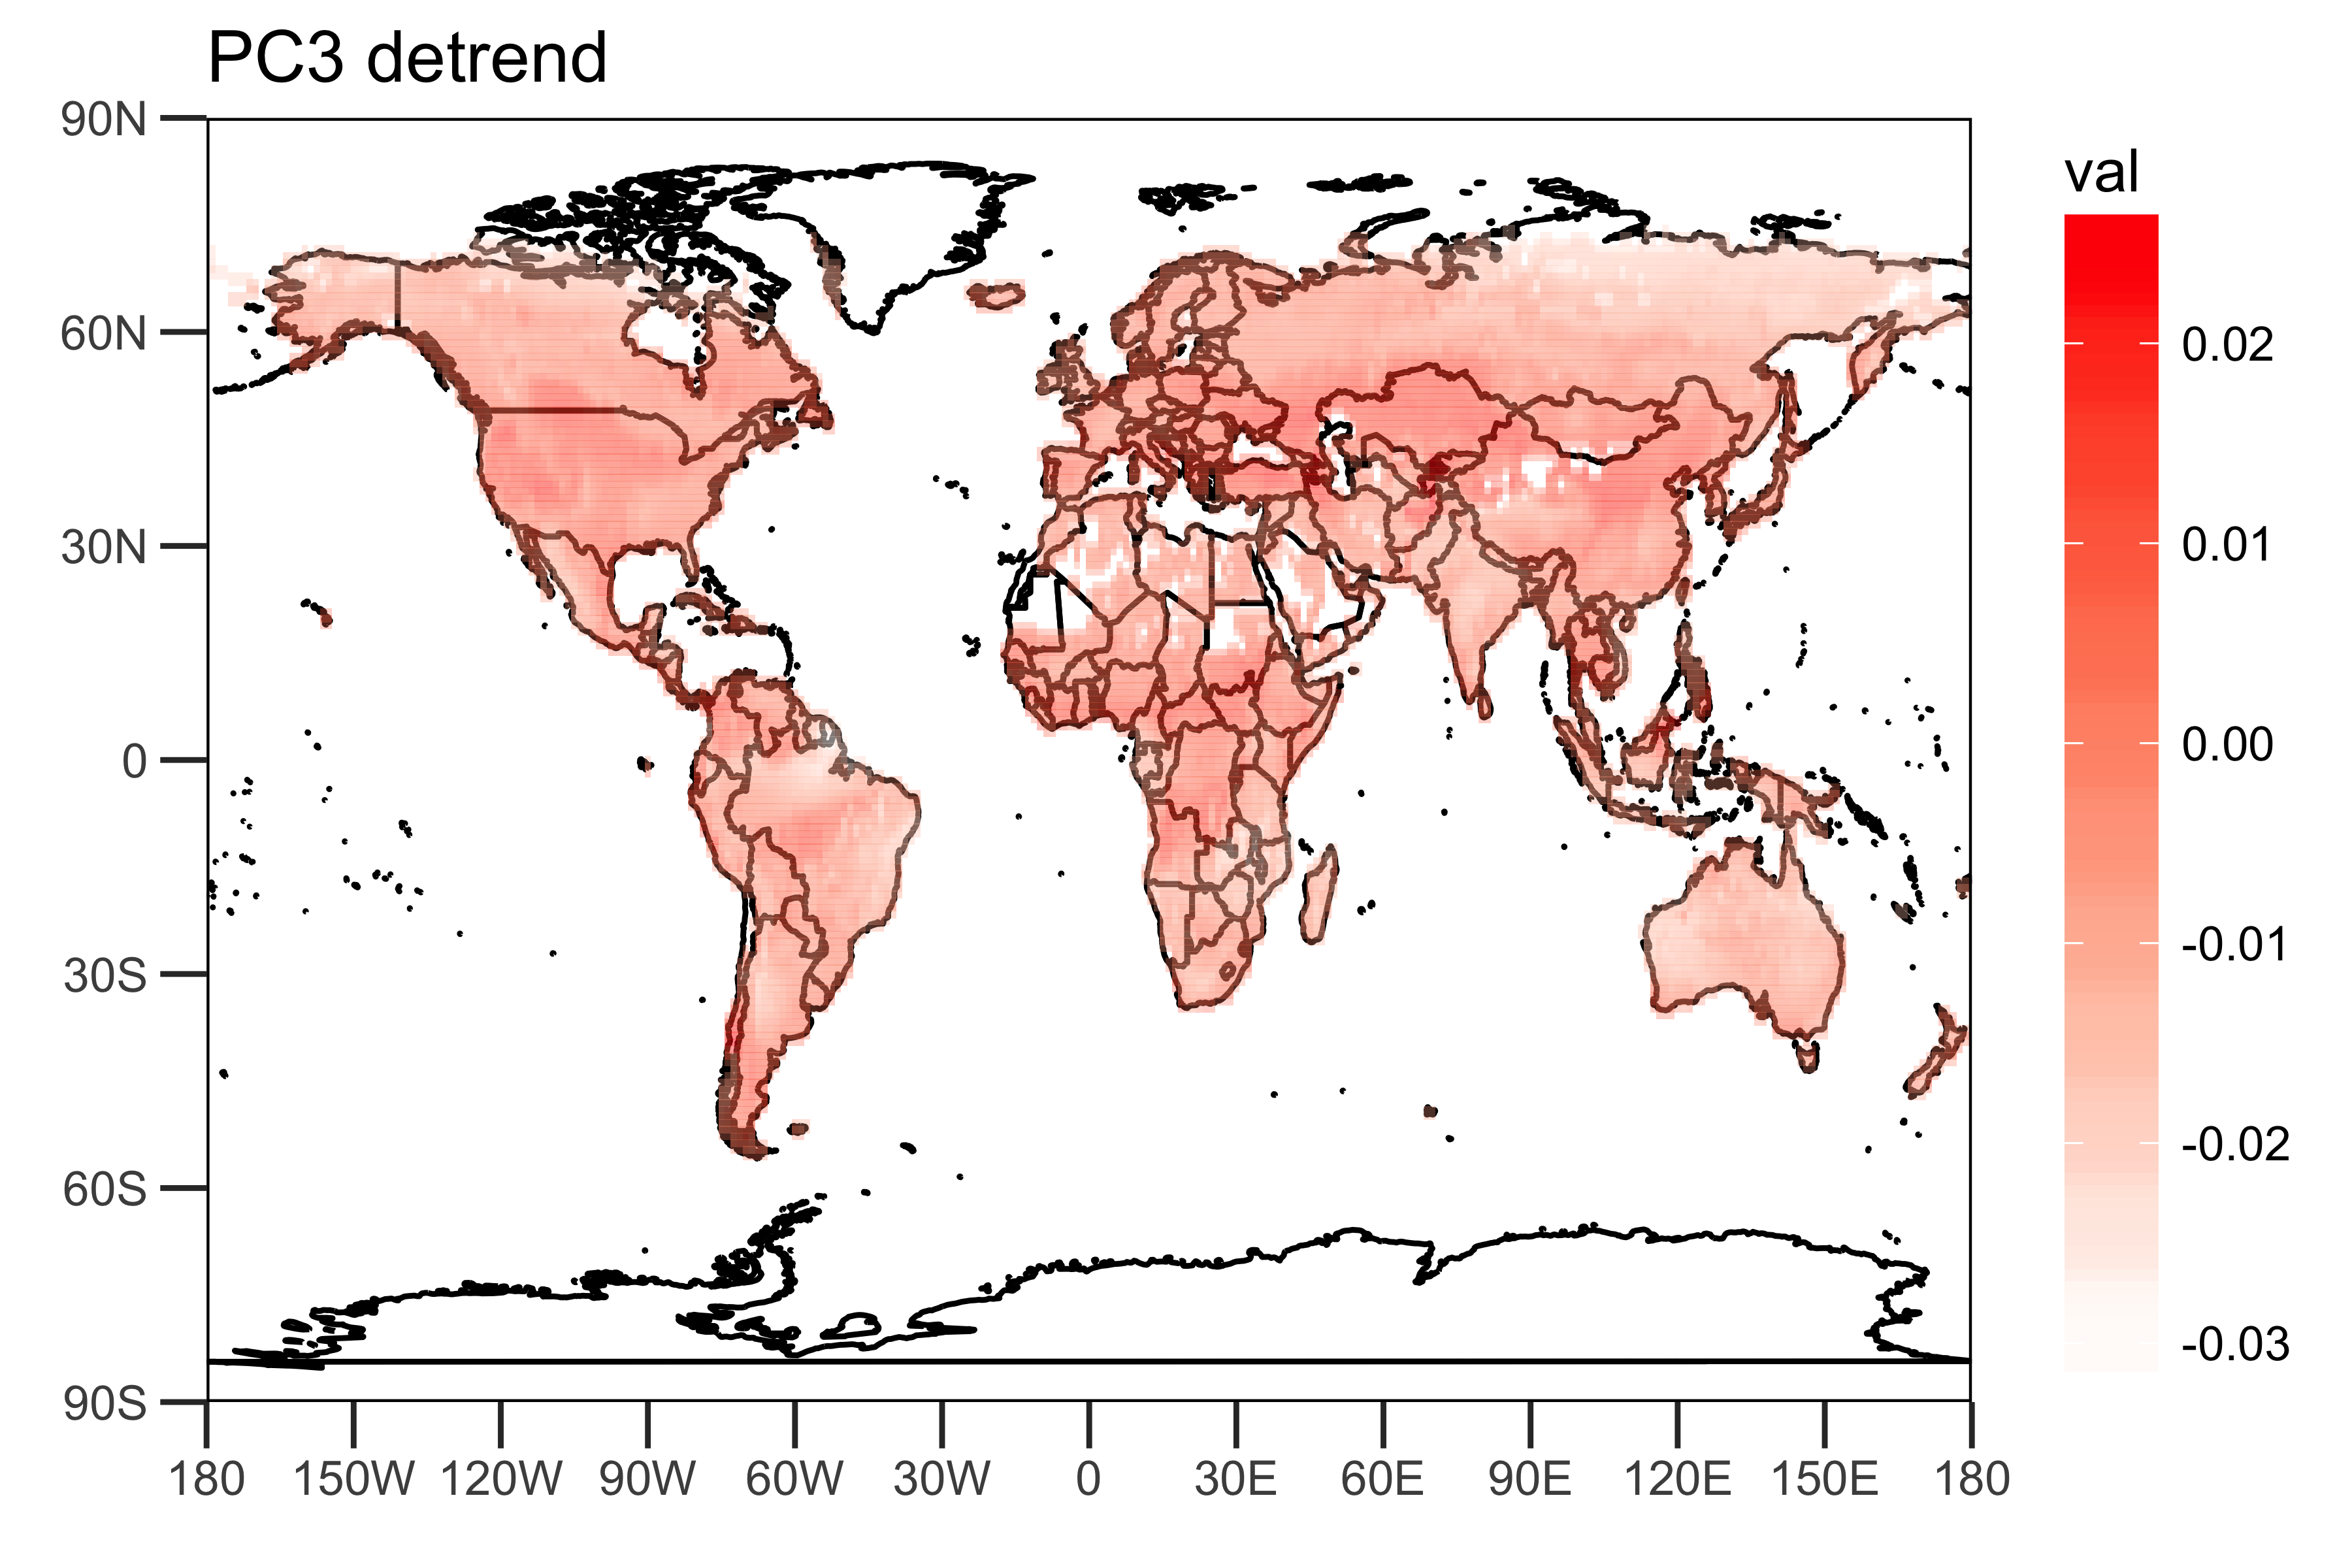
\includegraphics[width=0.9\linewidth]{../img/loading_PC3_de}
	\caption{Loadings of Principal Component 3}
	\label{fig:loadingpc3}
\end{figure}
\end{frame}

\begin{frame}
\frametitle{Principal Component Analysis}
\begin{figure}
	\centering
	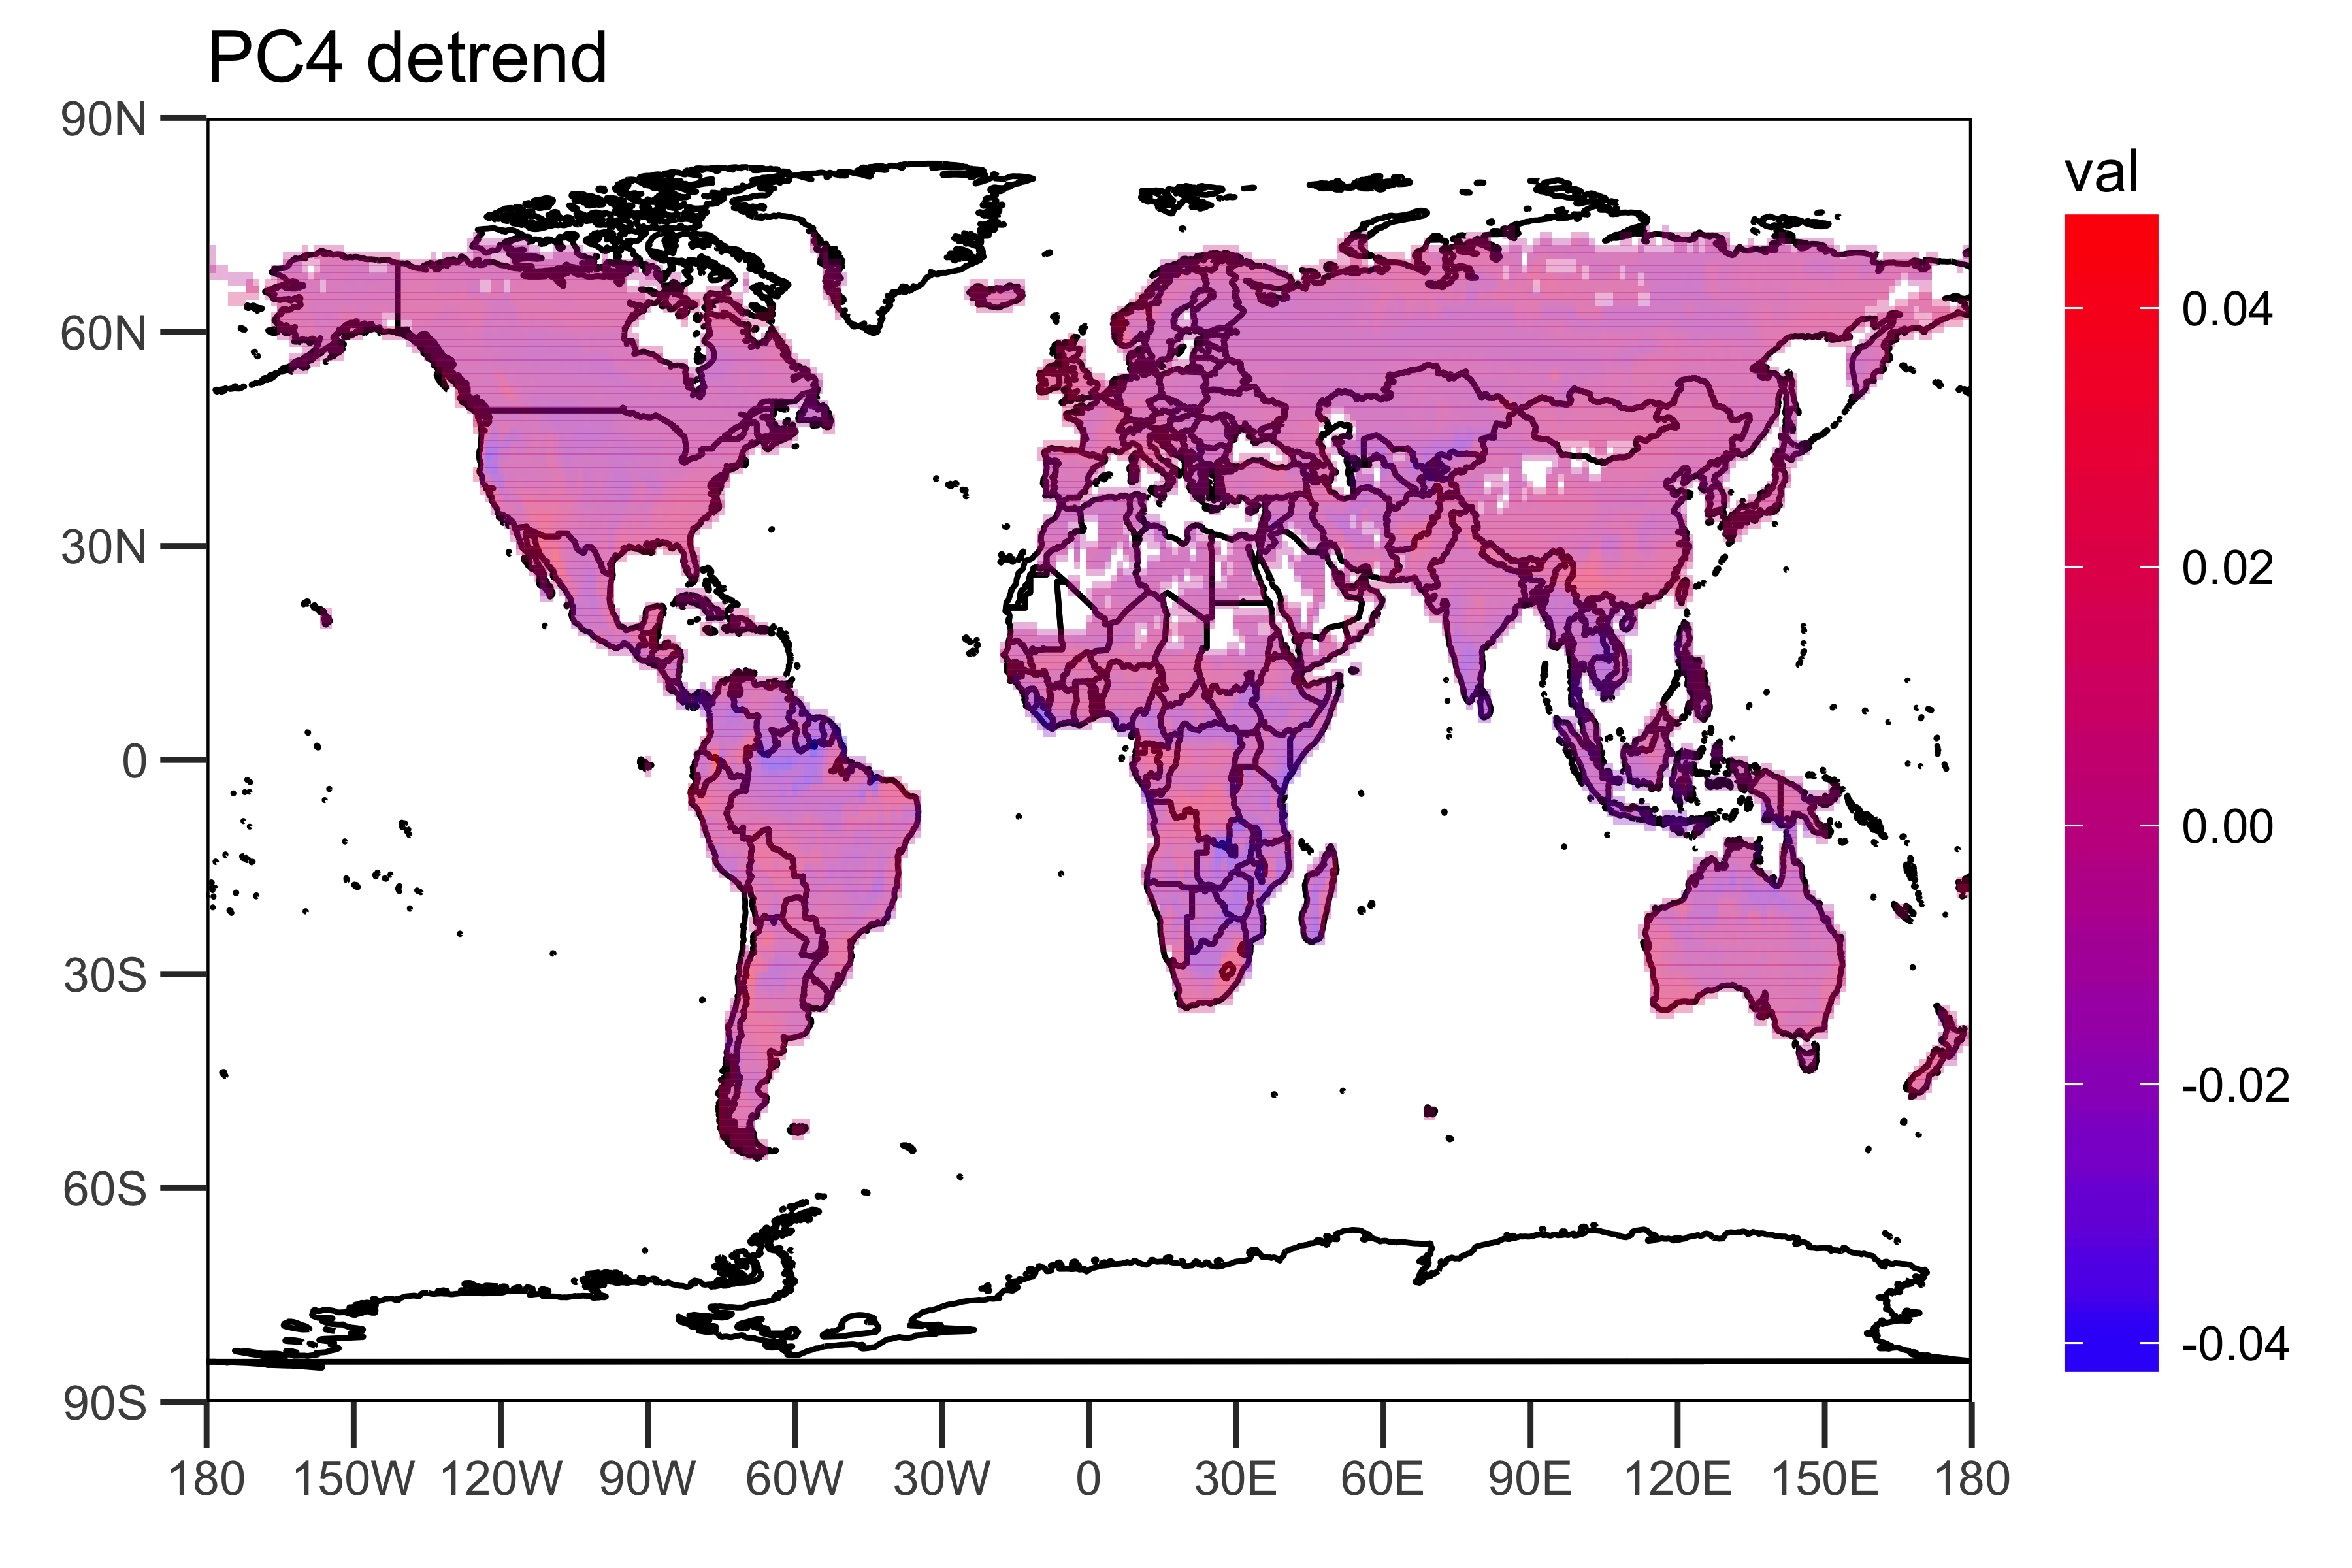
\includegraphics[width=0.9\linewidth]{../img/loading_PC4_de}
	\caption{Loadings of Principal Component 4}
	\label{fig:loadingpc4}
\end{figure}
\end{frame}

\begin{frame}
\frametitle{Principal Component Analysis}
\begin{figure}
	\centering
	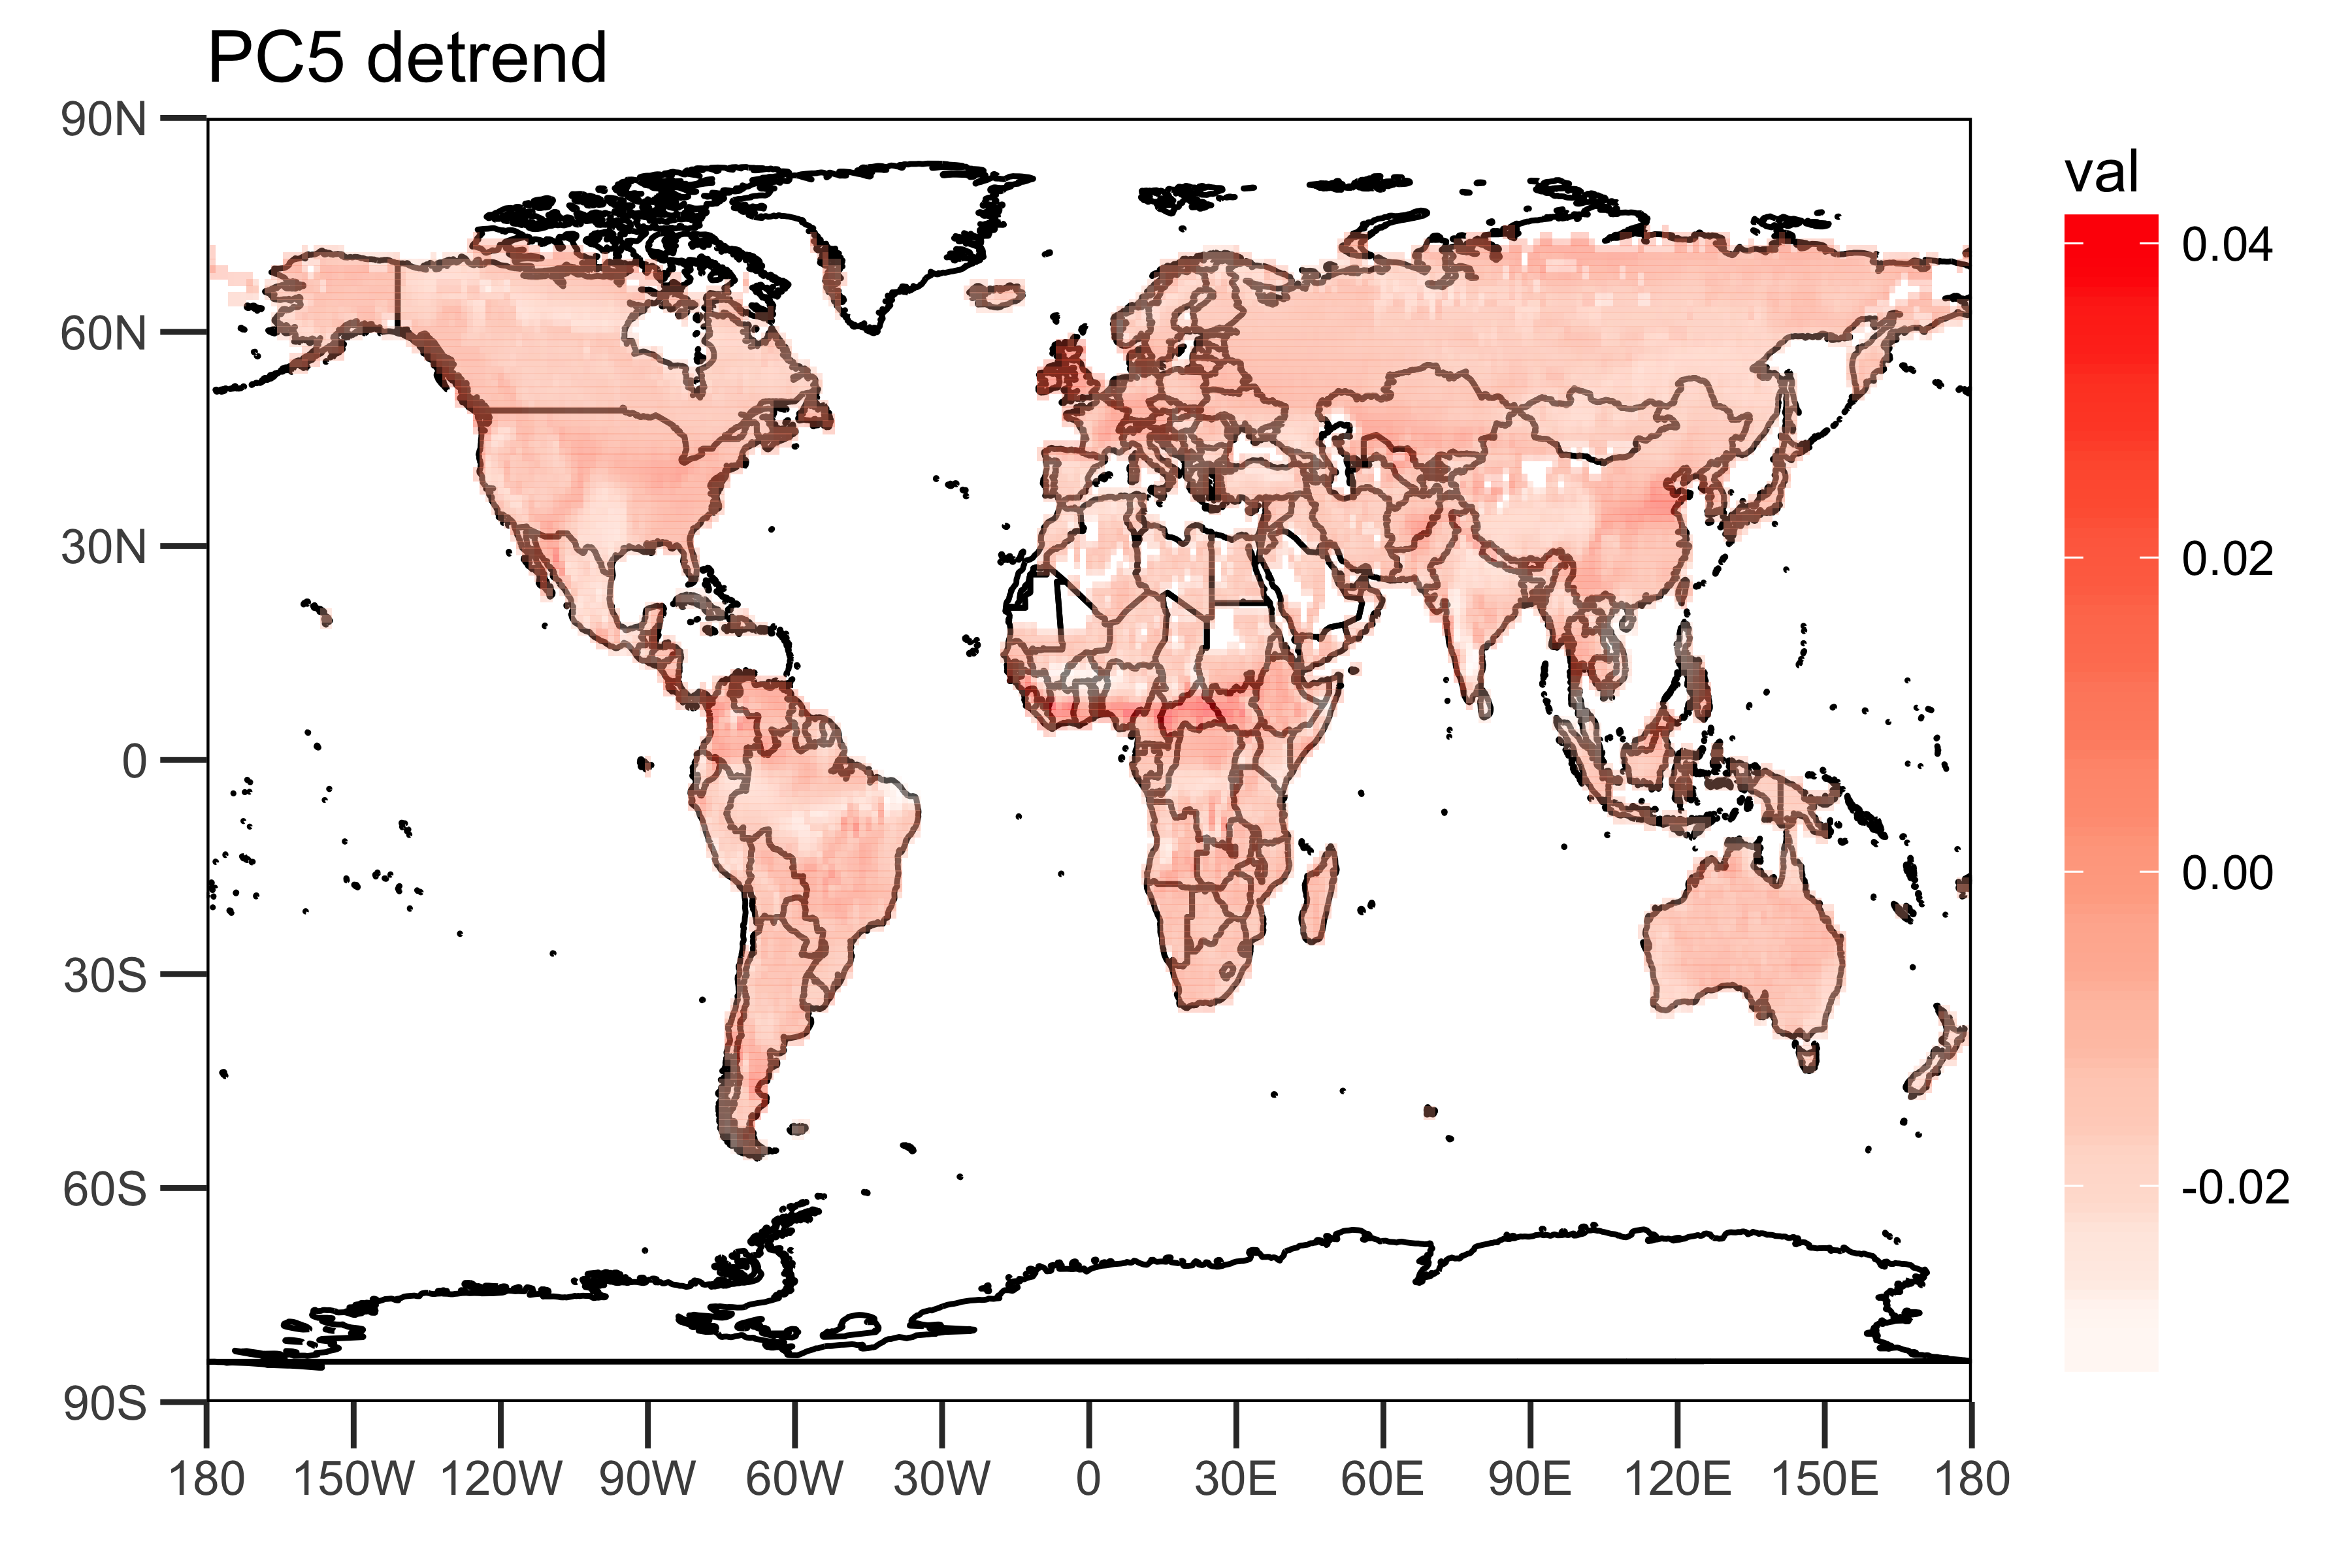
\includegraphics[width=0.9\linewidth]{../img/loading_PC5_de}
	\caption{Loadings of Principal Component 5}
	\label{fig:loadingpc5}
\end{figure}
\end{frame}

\begin{frame}
\frametitle{Principal Component Analysis}
\begin{figure}
	\centering
	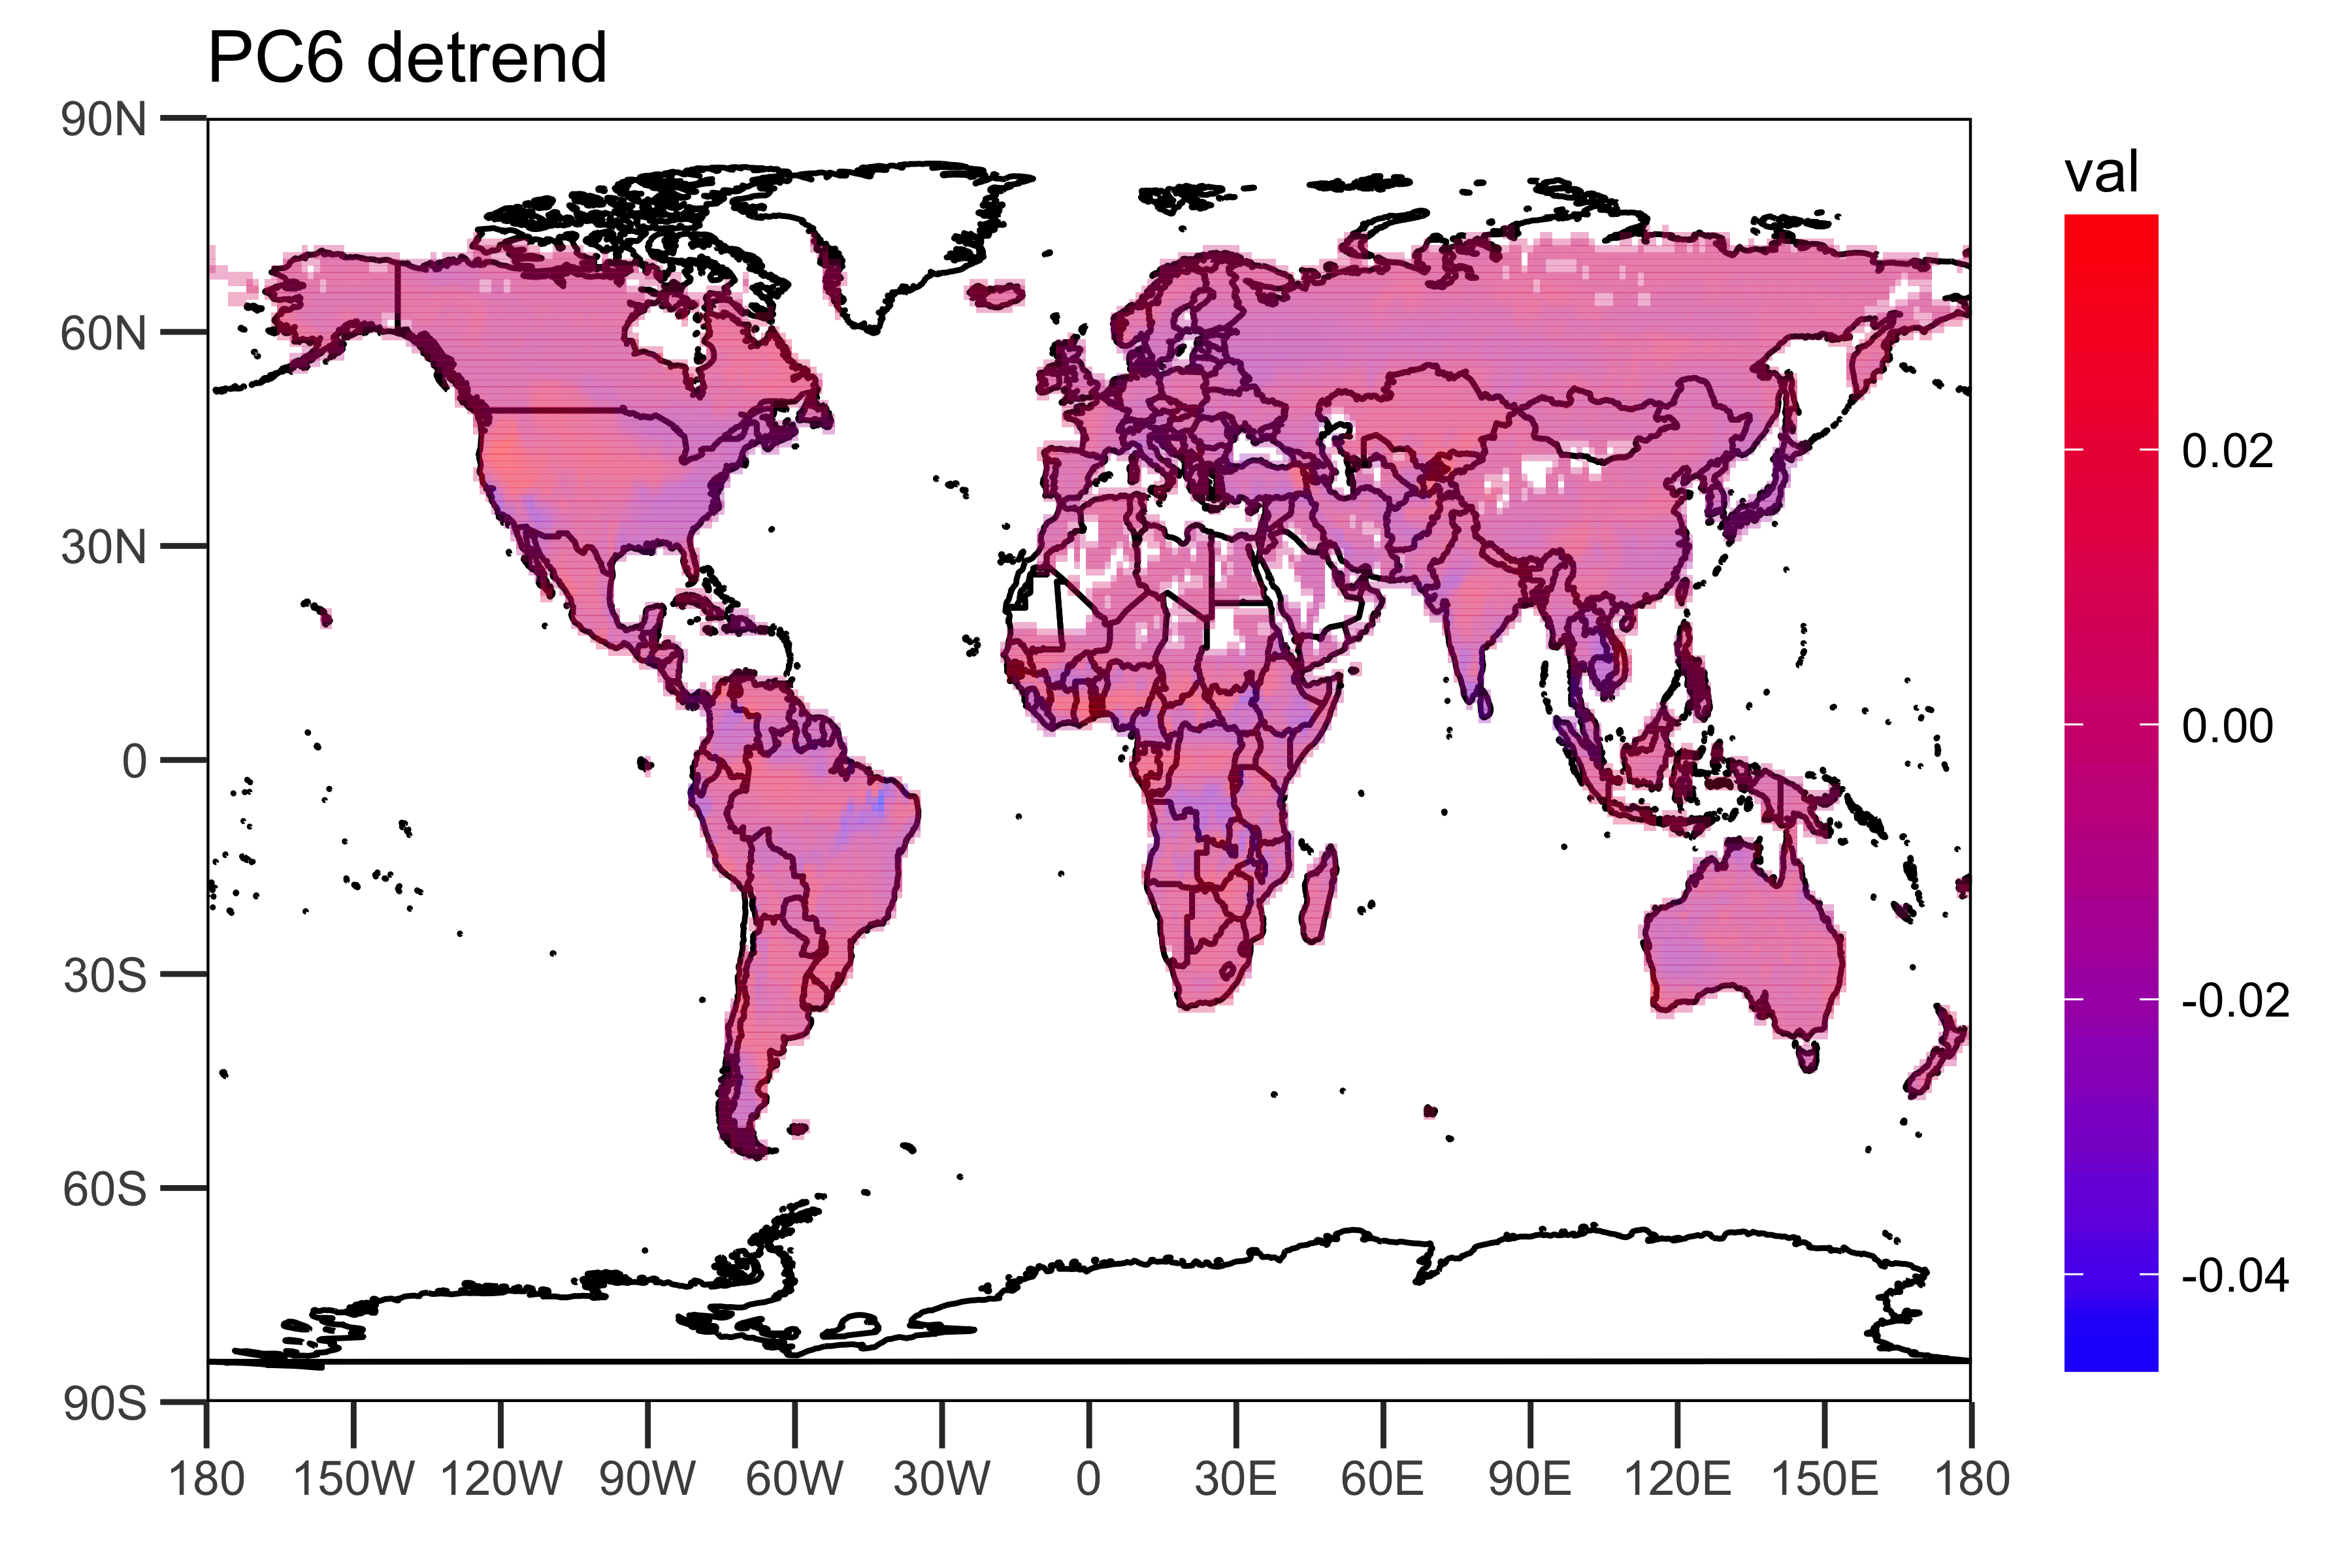
\includegraphics[width=0.9\linewidth]{../img/loading_PC6_de}
	\caption{Loadings of Principal Component 6}
	\label{fig:loadingpc6}
\end{figure}
\end{frame}

\begin{frame}
\frametitle{Principal Component Analysis}
\begin{figure}
	\centering
	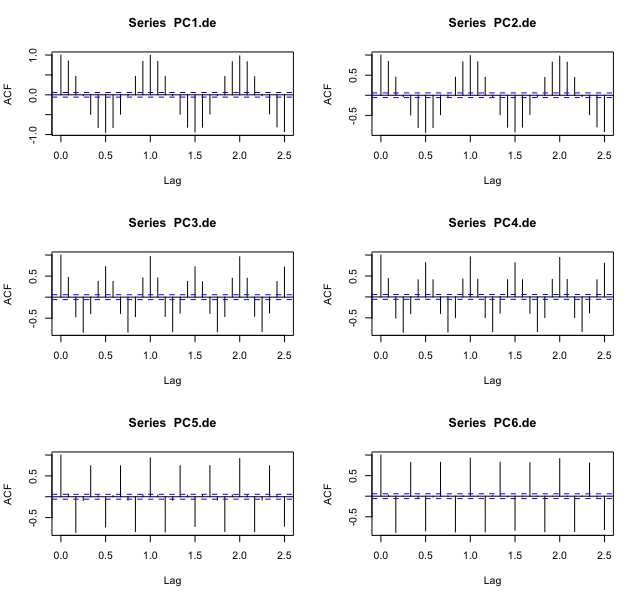
\includegraphics[width=0.7\linewidth]{../img/PCAde_ACF}
	\caption{Auto-Covariance Function}
	\label{fig:pcadeacf}
\end{figure}
\end{frame}

\begin{frame}
\frametitle{Principal Component Analysis}
\begin{figure}
	\centering
	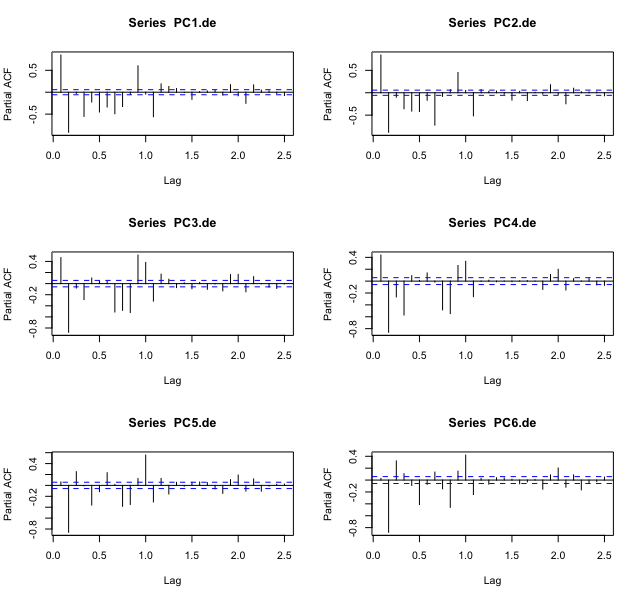
\includegraphics[width=0.7\linewidth]{../img/PCAde_pacf}
	\caption{Partial ACF}
	\label{fig:pcadpeacf}
\end{figure}
\end{frame}

\begin{frame}
\frametitle{Principal Component Analysis}
\begin{figure}
	\centering
	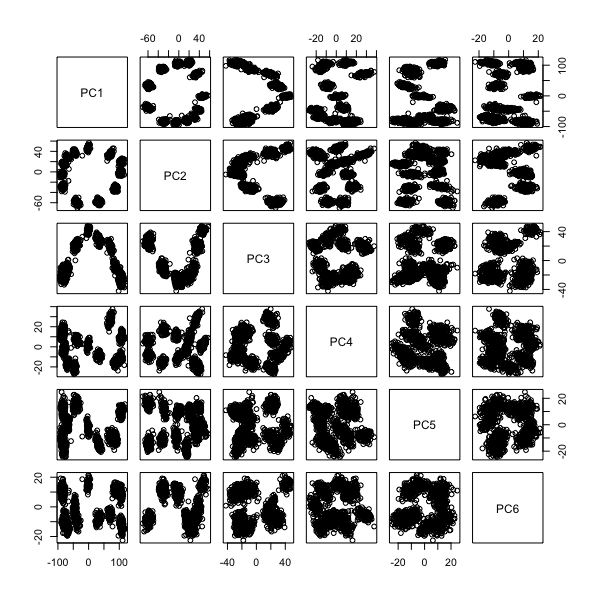
\includegraphics[width=0.7\linewidth]{../img/PCAde_pair}
	\caption{Pair Plot}
	\label{fig:pcade_pair}
\end{figure}
\end{frame}

\begin{frame}
\frametitle{Principal Component Analysis}
\begin{figure}
	\centering
	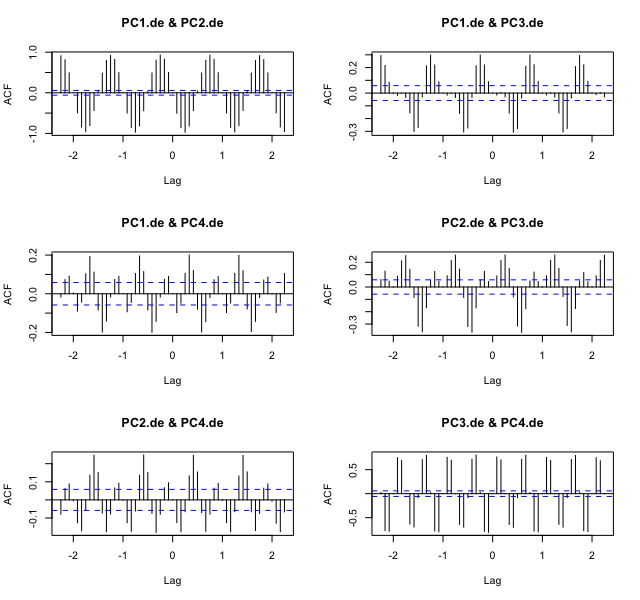
\includegraphics[width=0.7\linewidth]{../img/PCAde_CCF}
	\caption{Cross-Covariance Function}
	\label{fig:pcadpeccf}
\end{figure}
\end{frame}

\begin{frame}
\frametitle{PCA: Spectal Analysis}
\begin{figure}
	\centering
	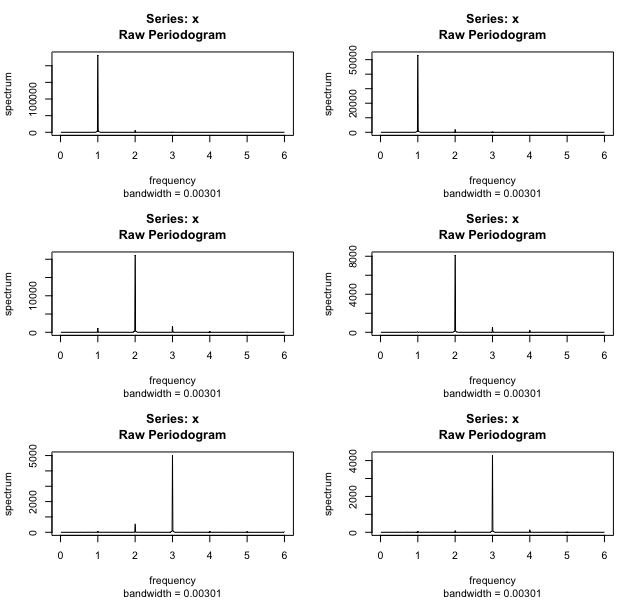
\includegraphics[width=0.7\linewidth]{../img/PCA_periodogram}
	\caption{Periodogram}
	\label{fig:pcaperiodogram}
\end{figure}
\end{frame}

\begin{frame}
\frametitle{PCA: Spectal Analysis}
\begin{columns}
	\column{2.5in}
	\begin{figure}
		\centering
		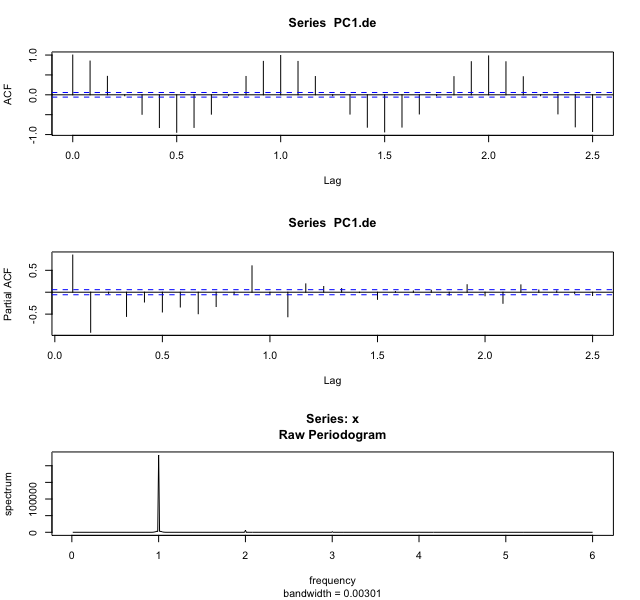
\includegraphics[width=0.7\linewidth]{../img/PCA_pc1}
		\caption{}
		\label{fig:pcapc1}
	\end{figure}
 \column{2.5in}
 \begin{align*}
 X_t &= A\cos(2\pi\frac{1}{12}t) + B\sin(2\pi\frac{1}{12}t)  \\ 
 &= R\sin(2\pi\frac{1}{12} + \varphi)\\
 & \text{ where } R^2 = A^2 + B^2, \\
 &\varphi = \arctan(\frac{A}{B}) \\
 \gamma(h) &= \sigma^2\cos(2\pi\frac{1}{12}h) \\
 \end{align*}
\end{columns}
\end{frame}

\begin{frame}
\frametitle{PCA: Spectal Analysis}
\begin{table}[ht]
	\centering
	\begin{tabular}{rrrrr}
		\hline
		& Estimate & Std. Error & t value & Pr($>$$|$t$|$) \\ 
		\hline
		cos(2 * pi/12 * 1:1140) & -32.6520 & 0.5834 & -55.97 & 0.0000 \\ 
		sin(2 * pi/12 * 1:1140) & -97.1938 & 0.5834 & -166.61 & 0.0000 \\ 
		\hline
	\end{tabular}
\end{table}
\begin{itemize}
	\item Residual standard error: 13.93 on 1138 degrees of freedom
	\item Multiple R-squared:  0.9645,	Adjusted R-squared:  0.9644 
	\item F-statistic: 1.545e+04 on 2 and 1138 DF,  p-value: < 2.2e-16
\end{itemize}
\end{frame}

\begin{frame}
\frametitle{Final Remarks}
\end{frame}

\end{document}
